\subsection{Metodo e formalismo di specifica}
L'architettura del progetto verrà esposta seguendo il metodo \gls{top-down}, si partirà, cioè, dal livello più generale per poi scendere nel dettaglio. I diagrammi di classe, attività e sequenza saranno conformi al formalismo \gls{UML} 2.x, come previsto nelle \textit{Norme di Progetto v3.0.0}.

\subsection{Architettura generale}
L'architettura del prodotto che vogliamo realizzare segue il pattern three-tier, che prevede la suddivisione dell'applicazione in tre diversi strati. I tre strati sono dedicati rispettivamente all'interfaccia utente, alla logica funzionale e alla gestione dei dati persistenti e comunicano tra loro secondo le linee generali del modello client-server. L'architettura three-tier\footnote{Si rimanda alla sezione \ref{pattern} per maggiori informazioni} permette una maggiore scalabilità e manutenibilità dell'applicazione in quanto è possibile modificare o sostituire uno strato indipendentemente dagli altri.

Attraverso la seguente figura presenteremo i tier dell'architettura adattati al nostro progetto, che saranno approfonditi nel dettaglio nelle sezioni successive del documento.

\begin{figure}[h]
	\centering
	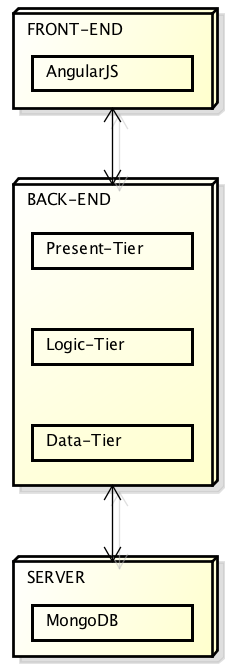
\includegraphics[height=0.6\textheight]{img/architettura_generale}
	\caption[Architettura generale del sistema]{Architettura generale del sistema}
\end{figure}

\textbf{Presentation-Tier}: contiene il \gls{front-end} dell'applicazione, che si occupa della presentazione dei dati all'utente. Funge da interfaccia tra l'utente e il \gls{back-end}, interagendo con il tier sottostante.

\textbf{Logic-Tier}: contiene il \gls{back-end} dell'applicazione. Comunica con il livello superiore elaborando le richieste generate da esso e recuperando i dati dal livello inferiore. 

\textbf{Data-tier}: questo livello è costituito dal \gls{database} dell'applicazione ed è dove vengono memorizzate e recuperate le informazioni. Nel nostro caso il \gls{database} è di tipo non relazionale.
